\documentclass[a4paper,12pt]{report}

% The following makes latex use nicer postscript fonts.
\usepackage{times}
\usepackage[english]{babel}
\usepackage{csquotes}% Recommended
\usepackage{amsmath,amsfonts,amssymb}
\usepackage{graphicx}
\usepackage[colorlinks,urlcolor=blue,linkcolor=blue]{hyperref}
\usepackage[backend=biber, style=apa]{biblatex}
\DeclareLanguageMapping{english}{english-apa}
\usepackage[section]{placeins} % To keep floats within their sections
\usepackage{vubtitlepage}
\usepackage[Rejne]{fncychap}
\usepackage{subcaption}

%\usepackage{layouts}
% TODO this is totally a thing
\graphicspath{ {images/} }
%\addbibresource{bib/Mendeley.bib}
\addbibresource{bib/Thesis.bib}
\addbibresource{other.bib}

% Tiny bit of extra whitespace, easy on the eye
\renewcommand{\baselinestretch}{1.05}
% Away with indents before paragraphs
\setlength{\parindent}{0pt}

\renewcommand*\rmdefault{bch}
% Yoni uses this one it's pretty but slim
% \renewcommand*\rmdefault{lmr}


% Redefine \paragraph to be sexier
\makeatletter
\renewcommand{\paragraph}{%
  \@startsection{paragraph}{4}%
  {\z@}{1.75ex \@plus 1ex \@minus .2ex}{-0em}%
  {\normalfont\normalsize\bfseries}%
}
\makeatother

\newcommand{\forceindent}{\leavevmode{\parindent=1em\indent}}


\begin{document}

\author{Ruben Vereecken}
\title{Dealing with the Dimension of Time in Deep Reinforcement Learning}

\promotortitle{Promotor}
\promotor{Prof. Dr. Ann Now\'{e}\\
Prof. Dr. Peter Vrancx}
\faculty{Faculteit Wetenschappen en Bio-ingenieurswetenschappen}
\department{Departement Computerwetenschappen}
\reason{
\small
Proefschrift ingediend met het oog op het behalen van de graad \\
van Master in de Ingenieurswetenschappen: Computerwetenschappen
}
\date{August 2016}

% First dutch TitlePage
\maketitlepage

\faculty{Faculty of Science and Bio-Engineering Sciences}
% \advisortitle{Begeleider}
\department{Department of Computer Science}
\reason{
Thesis submitted in partial fulfillment of the requirements \\
for the degree of Master in Applied Sciences and Engineering: Computer Science
}

\date{Augustus 2016}

% Then english TitlePage
\maketitlepage


\pagenumbering{roman}
\tableofcontents

% Actual content

\pagenumbering{arabic}
\chapter{Introduction}

\label{introduction}
Reinforcement Learning is what we have labelled the remarkable ability of man and beast alike 
to learn from their surroundings and their interactions with it.
It is embodied in our learning from past mistakes or our failing to do so.
For quite some time now people have attempted to bestow this same ability to 
our computing devices so that they would figure out how to tackle problems by themselves
without explicit instructions.
While the field has not been without success
it has been slow going,
crawling forward inches instead of the hoped-for leaps.

A great effort has been put forward by DeepMind with their DQN [TODO].
Through the combination of great research and sufficient computation power
their reinforcement learners have managed to beat humans
on a great array of Atari games.
Still, some games remain largely or completely unbeaten.
It is my goal to investigate their shortcomings
and supplement them with new techniques in the domain
in order to point out which direction of research
offers the most interesting insights and rewards
to further the field of Reinforcement Learning. 
\chapter{Machine Learning}

\section{Introduction}
The world of today is generating huge amounts of data
as it goes along,
and more and more of it is put to use.
It is quite probable that any consumer in our society
that goes shopping,
uses some kind of service,
or uses the internet
on a daily basis
performs actions that end up in a database.
Not only do persons generate data,
so does everything else we monitor,
and our society happens to monitor quite a lot.
This data is invaluable for any organization that benefits
from information,
and truly, most do.
It is used by financial institutions like insurance companies,
medical institutions, commercial companies, scientific research
and everything in between.
Evidently, as the need for knowledge (or awareness thereof)
increases, so must our abilities to uncover it,
making machine learning an incredibly interesting topic
in today's world.

People are good at creating hypotheses
about what things mean,
connecting the dots
and predicting cause or outcome.
Yet we can only cope
with so much data at a time
and without direction,
the answers we seek may elude us.
Enter the computing device,
programmable to our needs.
Computer programs often take the form
of our expert knowledge put to detailed writing
but they can also cover the gaps where
we don't have the knowledge
and instead need to uncover it.
This includes anything of valuable information to us,
be it patterns in certain data or hypotheses for predictions.
Where the domain expert describes such hypotheses
using a computer program,
the machine learning expert devises ways of uncovering
the hypotheses.
Evidently, the power of computers would be much greater
if they would be made able to learn as we do.

Great advances have already been made in the domain,
yet we have not managed to make computers learn
as well as humans do,
at least not in as many regards as we do.
The best applications do, however,
get better results than humans in very specific domains.


\paragraph{}
Machine learning is a collection of methods
used to bridge the aforementioned gap
between data and knowledge.
A machine learning algorithm learns from data
and learns an hypothesis or model on it,
which can then be used to make predictions on future data.
This separates it from other algorithms
designed by an expert
that follow a static rule set.
It is inherently an interdisciplinary field,
with its roots firmly embedded
in a statistical foundation
combined with AI,
drawing inspiration from fields such as
information theory,
complexity theory,
psychology
and other fields.

The rest of this chapter will describe the basics of machine learning
along with the specific tools I will use throughout this thesis.
The foundation should be quite sufficient to build up
an understanding of the field
so as to allow the reader to follow the following chapters comfortably.
Next to exploring a foundation,
I will describe specific methods such as neural networks
and convolutional layers,
both exciting techniques that will be used further on.
However, perhaps to the reader's delight,
a cursory glance at the high-level introduction of these methods
should suffice for the reader who only seeks to understand
the applications described herein.
The careful reader is of course cordially invited
to read the more detailed descriptions.


\section{Hands-on Introduction}
A machine learning algorithm
is usually required to form hypotheses
based on given observations.
In this way it can be seen as
a black-box oracle
in which data are shoved
and answers pop out.
Let's take as an easy example
the probably overused and dead-beaten weather forecast.

Let's say we only need to do a daily forecast.
Data come in in the form of meteorological observations
such as temperature, wind speed, and whatever else
experts observe to make top-notch predictions.
This then gets paired
with a description of the actual weather the next day.
Together they form experience-target pairs
$(x_i, y_i)$
that correspond to a meteorological observation
on the one day and the weather on the next day,
in the hope that we can somehow deduce the hidden
link between the two.
The target $y_i$ is what we're really after
so we should choose carefully as to what we are trying to predict.
$y_i$ can be a nominal value,
i.e. from a given set of values
such as the set $(sunny, rainy, windy)$,
in which case the problem is called a \textit{classification} problem.
Contrarily, it can be a real-valued number such as temperature
in which case we call the problem a \textit{regression} problem.
The distinction is worth noting because
some techniques lend themselves well to
one category but not necessarily to the other.
On this data we will try to learn a hypothesis $h$
that can predict the target weather $y$
for any given observation $x$.
Now all we need to do is fill in the bits in between.

We already have a vague description of what we want to achieve
but now we need to design the problem.
Let us pick for our targets the real-valued temperature on a given day.
The observations, or \textit{features}, we will base our model on
will take the form of a vector
$(Temperature, Sky, Wind)$ or $(x_1, x_2, x_3)$ short,
where $Temperature$ and $Wind$ are real-valued,
whereas $Sky$ takes on one of the three values
$(Sunny, Rainy, Cloudy)$.
Now we need some kind of function connecting
observation to target.
One of the easiest choices would be a linear
function that combines the features
and outputs the target we are looking for.
It would look quite simple:

$$ y = w_0 + w_1x_1 + w_2x_2 + w_3x_3 $$

We are still stuck with the problem that $x_2$, or $Sky$,
is a nominal value and therefore does not fit all too well with algebra.
We can work around this by agreeing on
a little preprocessing step
that maps $Sunny$ to $-1$, $Rainy$ to $0$ and $Cloudy$ to $1$.
Now that our model is defined, all that is left for us to do
is train it.

In order to train our model we need a data set with training examples
$(x_i, y_i)$,
where the temperature $y_i$ corresponds to
the observations $x_i$ the previous day.
All that remains now is to pick the best weights
so the resulting model is the best hypothesis.
We describe a \textit{best fit}
we need some metric of performance.
The easiest one available is the error on the predictions made by the model
compared to the targets in the training data.
The best hypothesis is the one that minimizes this error.
The most common error by far is the \textit{mean squared error},
though others certainly exist.
Given a training set $D$, it is defined as follows:

$$ E = \frac{1}{|D|} \sum_{(x_i, y_i) \in D}{(h(x_i) - y_i)^2} $$

Multiple algorithms exist that minimize $E$ in such a manner.
If all data is available in one go, as it is in our case,
we can simply apply linear regression to our system
of $|D|$ equations $y = xw$ in order to find a $w$
with the lowest error.

\subsection{Finishing up the example}
An alternative algorithm to find our optimal weights $w$
is the \textit{weight update rule},
a source of inspiration for many more algorithms.
The idea behind is that every sample
you calculate your prediction
and shift the weights in the direction of the error,
proportionally to the size of the error.
So, for every sample:
\begin{enumerate}
\item Calculate $\hat{y_i} = h(x_i)$
\item Update $w_i = w_i + \eta(y_i - \hat{y_i})x_i$
\end{enumerate}

The update size can be tweaked with $\eta$.

\paragraph{}
As you have witnessed yourself,
designing a machine learning task
is rather an art than an exact science.
The first optimization algorithm proposed,
linear regression,
is only available for linear models.
Finding the ultimate weights
makes more sense in a regression context
as opposed to a classification context.

There are many more such decisions to made
and models to choose from.
During the next sections,
I will touch on some interesting
models that are used throughout this thesis.

\section{Underfitting and Overfitting}
Why not just go for an error of $0$?
We could, however it is unlikely since we suffer from two problems:
insufficient data and a delusion of a perfect world.
In other words, our features probably are not sufficient
and our data is noisy.
If we still manage a training error of $0$
we probably committed the grave mistake of
\textit{overfitting} the training data,
meaning we included the noise of the data in our model.
The reason this is to be avoided is that by definition
noise cannot be predicted and a model that tries
to do so will perform even worse on similar unseen samples.

\paragraph{}
Figure
\ref{fig:overfitting}
demonstrates this phenomenon of overfitting.
A high-dimensional polynomial is fitted on
a small set of samples drawn from a noisy
distribution that follows a goniometric function.
The model that we would like to attain
should be as close as possible to the original function.
However, if we try to fit the available data completely,
the polynomial results in a model that performs
well in the very close vicinity of the training points
but performs horrendously on unseen data
that deviates from the original training data.
This can be seen from the discrepancy
between the model and true function.
It follows that overfitting is characterized by
a low training error but a high generalization error,
or put otherwise,
the model fails to generalize the training data.

\begin{figure}[h]
\center
\begin{subfigure}{.49\textwidth}
  \centering
  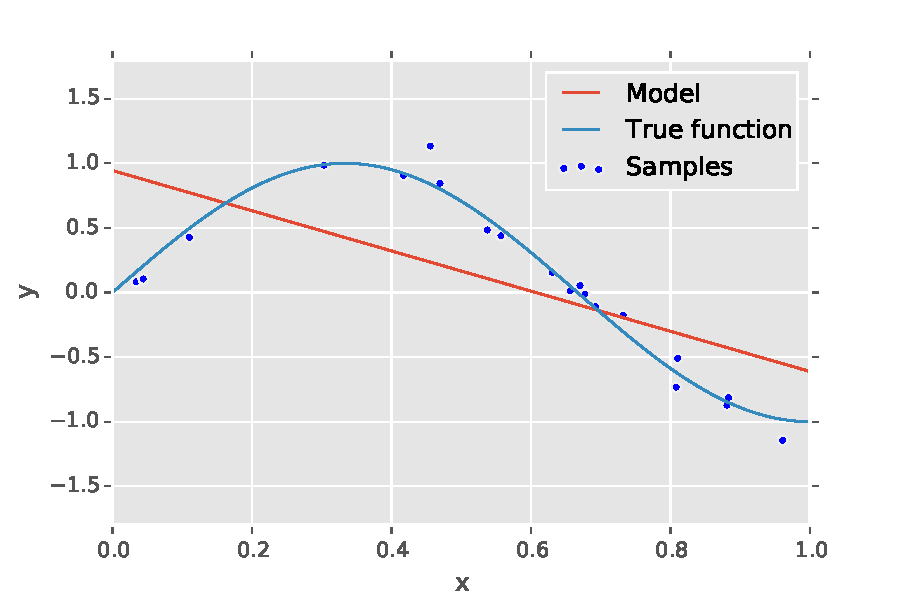
\includegraphics[width=\textwidth]{underfitting.pdf}
  \caption{Underfitting}
  \label{fig:underfitting}
\end{subfigure}
\begin{subfigure}{.49\textwidth}
  \centering
  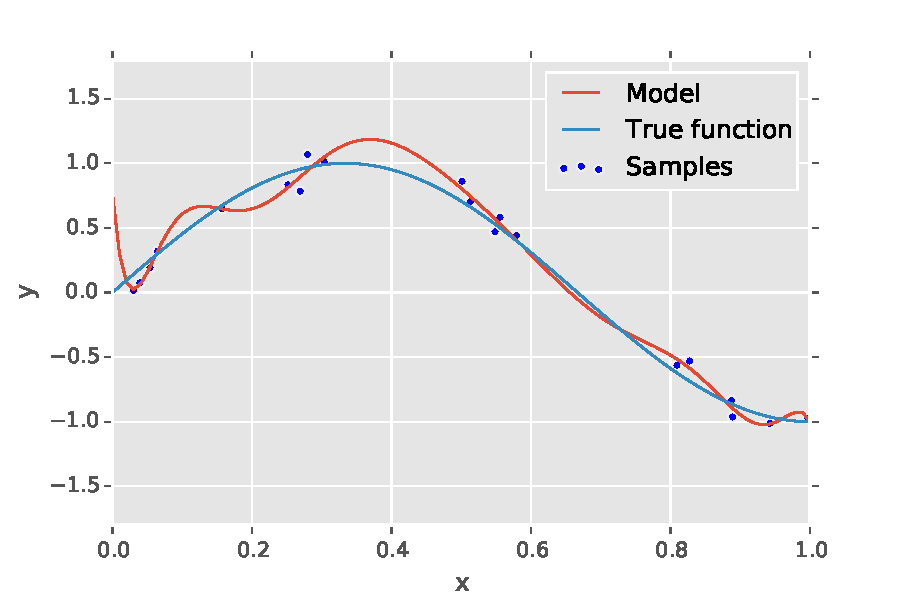
\includegraphics[width=\textwidth]{overfitting.pdf}
  \caption{Overfitting}
  \label{fig:overfitting}
\end{subfigure}

\label{fig:fitting}
\caption[Underfitting and Overfitting]{
Underfitting and overfitting
demonstrated with two polynomial
models on noisy data modeled
after a goniometric function.
}
\end{figure}

The opposite of overfitting would then be \textit{underfitting},
as demonstrated by Figure \ref{fig:underfitting}.
This is often the case for models that lack
representational power
no matter how much data is available.
While the figure contains a rather naive example
of a 1-dimensional polynomial fit,
it illustrates perfectly how some models
can never hope to attain a complex underlying function.

It will not be possible to minimize the training error entirely,
though an underfitting model may still outperform
an overfitted one.

\paragraph{}
As should be clear from the example,
neither under- nor overfitting are good,
in fact an algorithm designer
should be weary of both.
It is best to explore multiple
algorithm settings in order to find
a model that is prone to
neither kind of misfitting.

In the next section I will describe a measure
that helps guide this search.

\begin{figure}[h]
\center
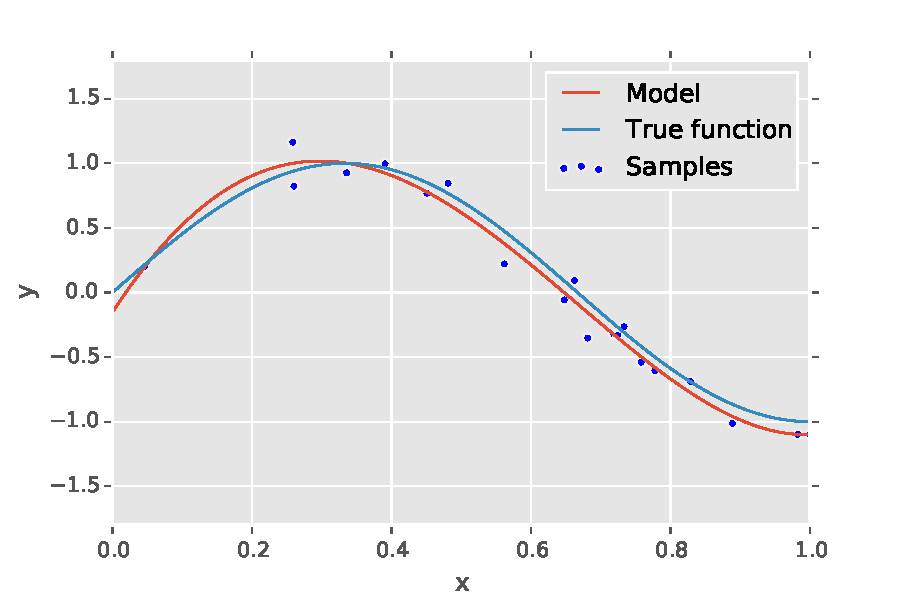
\includegraphics[width=.7\textwidth]{perfectfitting.pdf}
\label{fig:perfectfitting}
\caption[Curve fitting]{The right model can perfectly generalize from noisy data,
insofar as the data covers the desired domain}
\end{figure}

\section{Bias and Variance}
A common way to describe a learning algorithm
is in terms of its
bias and variance.
They are two different sources of error
the algorithm designer wishes to minimize.
The \textit{bias} of a learning algorithm
is the error inherent to the algorithm
because of false assumptions,
such as an unsuitable degree for a polynomial model
in the previous example.
This does not necessarily mean the model is weak on its own,
it only is for a specific problem.
Bias gives cause to underfitting,
as can be seen in Figure \ref{fig:underfitting}.

Bias can be quantified as the difference
between the expected prediction
and the true function value:

$$
\text{Bias}(x) = E[\hat{f} (x)] - f(x)
$$

\textit{Variance}
on the other hand,
is error because of sensitivity to noise:
small fluctuations in the data set.
It is the variability of a model's predictions.
As a result,
high variance may causes overfitting
noise inherent to the data but not to the model.
A typical example can be seen in Figure \ref{fig:overfitting}.

Variance can be quantified in terms of
the expected deviation of a prediction (variability):

$$
\text{Variance}(x) = E[ (\hat{f}(x) - E[\hat{f}(x)])^2]
$$

It can be lowered by
reducing the amount of features
(especially those of little import to the model)
or increasing the amount of data points.

\paragraph{}
Bringing these two notions together
gives us the \textit{bias-variance decomposition}
of a learning algorithm's generalization error,
i.e. the expected error on unseen data:

$$
\text{Err}(x) = E[(Y - \hat{f}(x))^2]
$$
$$
\text{Err}(x) = (E[\hat{f} (x)] - f(x))^2 + E[ (\hat{f}(x) - E[\hat{f}(x)])^2] + \sigma^2
$$

As you can see, the first two terms
are Bias squared and Variance respectively.
That leaves us with the last term
which is the irreducible error,
an error resulting from a lack of
omniscience; a lack of data.

From this decomposition we can see that we
can see that we can only have an error of 0
given the original model behind the data
an infinite amount of data. % bold claims man

\begin{figure}[ht]
\center
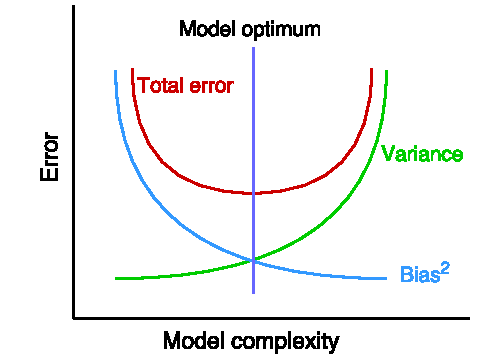
\includegraphics[width=0.7\textwidth]{bias_variance.pdf}

\caption{Bias-Variance decomposition}
\label{fig:biasvariance}
% TODO
\end{figure}

\paragraph{}
Figure \ref{fig:biasvariance}
visualizes the bias-variance decomposition
and shows the general tendencies of its individual components.
As bias decreases, variance generally goes up
and vice versa.
The goal of any algorithm designer
is then to find the sweet spot;
the model that optimizes the traded
between the two.

This can be done by exploring parameters
for a certain model,
like the degree of a polynomial,
and calculating the
\textit{expected generalization error}, % yes made this up myself lucid moment
since the true generalization error
is never known.
This in turn can be done
by keeping a separate test set
and calculating the error on that,
or other techniques that make clever use
of the training data
such as bootstrap or cross-fold validation.
I'll delve into those in the next section.

\begin{figure}
\center
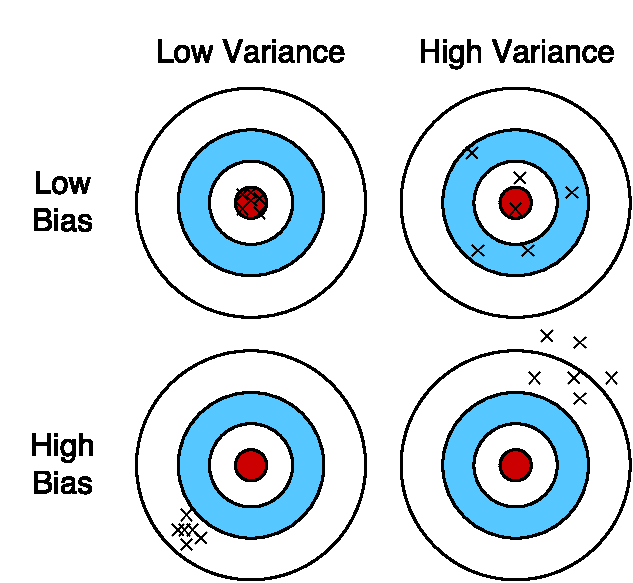
\includegraphics[width=0.7\textwidth]{dartboard.pdf}
\caption[Dartboard Analogy]{
  Dartboard Analogy
  \parencite{sammut2011encyclopedia}
}
\label{fig:bullseye}
\end{figure}

\paragraph{}
So far the discussion on the
generalization error and how to mitigate it,
I'd like to finish with a depiction
of bias and variance in Figure \ref{fig:bullseye}.
The center of the red target
is some target value $f(x)$
and darts are predictions $\hat{f}(x)$.
You can imagine this is the same x
for many instantiations of the same model
or it is a different x for every dart $\hat{f}(x)$,
it doesn't matter.

A high variance will have a scattering effect.
After all,
variance describes the variability of predictions.
High bias is the inability to generalize
well because of the model's false assumption:
in the image the model assumes an incorrect target.
The goal is once to have both measures as low as possible.

\section{Model Validation}
When training a model,
one typically wants to know the generalization error
as it is described in the previous section.
You already have the training error
because it is what you are trying to minimize,
but it usually generalizes poorly
to the generalization error.
It can actually be harmful to
watch only the training error during training,
so you need an indication of how the model
generalizes past training.

Often there are training, validation and test phases.
Validation is the stage
where we are trying to decide on the best model;
this is when model parameters are determined
(model selection).
During testing we simply see how well the model
is expected to generalize beyond experience.
At this point no more tuning is performed.
If the same data would be used for both validation
and testing,
the resulting test error
would probably be overly optimistic
\parencite{friedman2001elements}
since we are trying to determine prediction error
based on the data that was used to determine
the very model we are using.


\paragraph{}
A naive way to go about this
is to take a separate set of data
that comes from the same distribution
as the training data
(because otherwise your measure says very little
or your training data was chosen poorly)
and calculate the error of the model on this set.
This \textit{validation set} should be large enough
to be representative of the underlying distribution
but need not be as large as the original training set.
A common measure,
when dividing a data set,
is to keep 20\% to 30\% aside
for validation purposes.
If a test set is also required,
a good rule of thumb is keeping
50\% for training data
and dividing the other 50\%
equally over validation and test sets.

This way of splitting up data is far from ideal
because it requires that the validation data
not be used during training.
Data is however far too valuable for training,
we would rather not use it to simply
compute a measure of success.

\subsection{Cross-Validation}
Cross-validation or K-fold cross-validation
is by far the most popular validation technique.
Gone with the separate validation set
(I'll ignore testing for prediction error for now),
cross-validation testing solves
the problem of data scarcity by not using up
the data you desperately need for training.

\begin{figure}[h]
\center
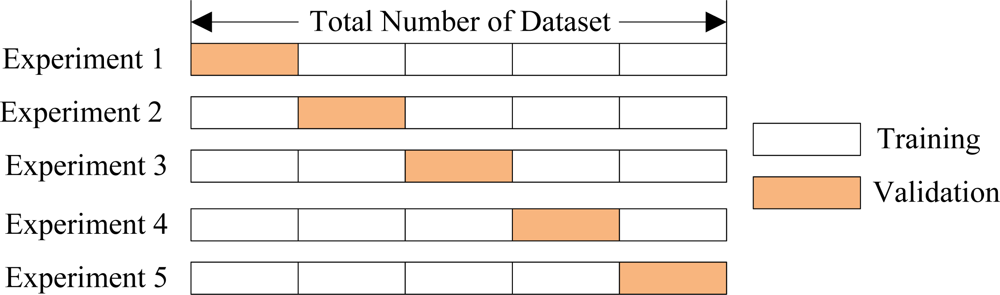
\includegraphics[width=0.8\textwidth]{crossval.png}
\caption[5-fold cross-validation]{
5-fold cross-validation
\parencite{Zhang2011}
}
\label{fig:crossval}
%TODO check attribution
\end{figure}

Figure \ref{fig:crossval} illustrates
how the training set is now divided into
K equal-sized \textit{folds}.
Each of these folds will be a validation set
in its own time.

The technique requires K
different models to be learned,
for a total of K iterations.
During iteration $i$,
fold $i$ is kept aside
as the validation set for this iteration
and all other folds together comprise
round $i$'s training set.

For each model the error is calculated on the validation
set, let's call this $\textit{CV}_i$.
The cross-validation error then becomes:

$$
CV(\hat{f}) = \frac{1}{N} \sum^{N}_{i=1} CV_i
$$

\paragraph{}
We now have a guess at the prediction error.
A good K is paramount for a good cross-validation error,
it also has a huge impact on the required amount of work
since computation time grows linearly with K.
We would like it to be quite low to save on computation time
yet high enough to have the cross-validation error
be a meaningful estimate.
Lower K tend to higher bias
because less data is used for training.
Higher K then tend towards
high variance.
This comes down to the same trade-off between
bias and variance,
though this time of an estimator
that estimates generalization error.
Generally good compromises for K are 5 and 10
\parencite{kohavi1995study}.

\section{Curse of Dimensionality}
The distance between two instances is calculated based on all of their attributes.
For these instances to have a small distance between them,
they should be close to one another in all of their attributes,
or otherwise put,
they should be similar in all aspects.
The more attributes or dimensions they have,
the harder this becomes.
This informally described phenomenon we call
the \textit{curse of dimensionality}.

\begin{figure}[ht]
\center

\begin{subfigure}{.49\textwidth}
  \centering
  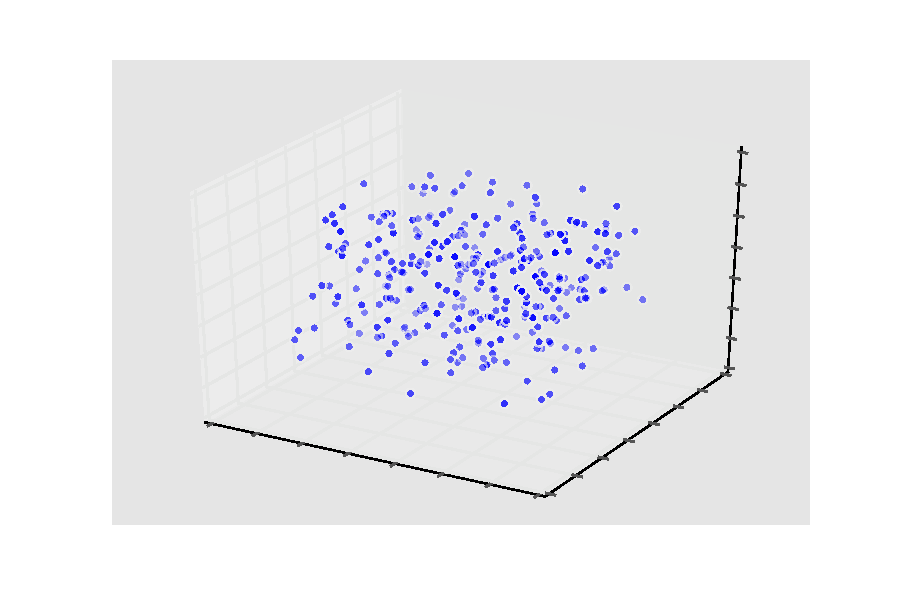
\includegraphics[width=\textwidth]{curse_3d.pdf}
  \caption{3 dimensions}
  \label{fig.ml.cod3}
\end{subfigure}
\begin{subfigure}{.49\textwidth}
  \centering
  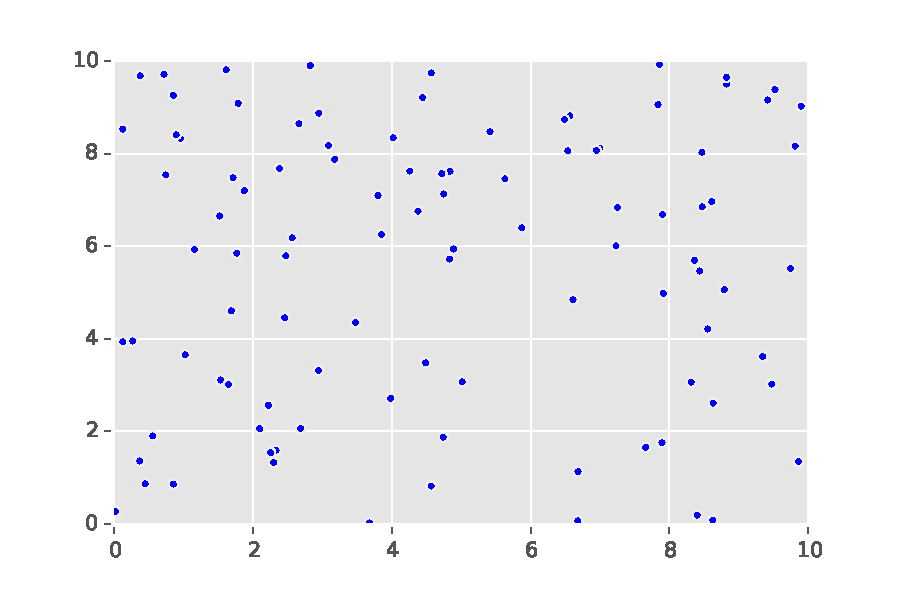
\includegraphics[width=\textwidth]{curse_2d.pdf}
  \caption{2 dimensions}
  \label{fig.ml.cod2}
\end{subfigure}
\begin{subfigure}{.45\textwidth}
  \centering
  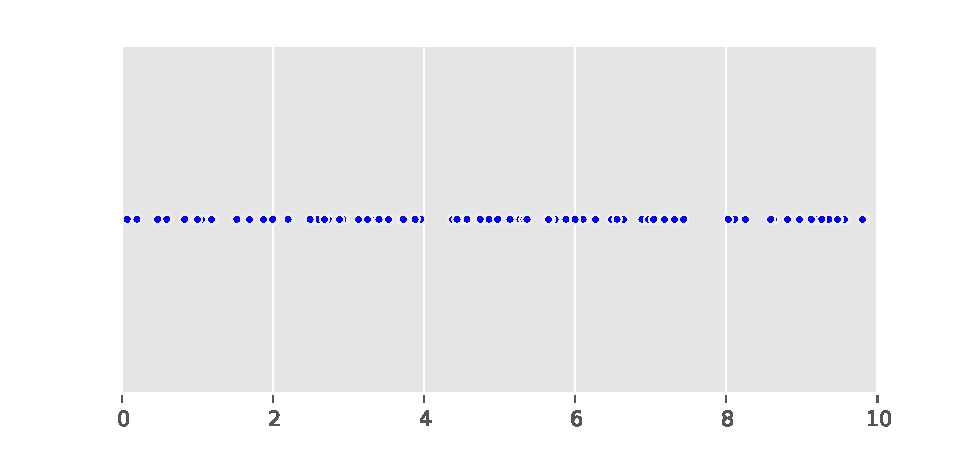
\includegraphics[width=\textwidth]{curse_1d.pdf}
  \caption{1 dimension}
  \label{fig.ml.cod1}
\end{subfigure}

\caption[Curse of dimensionality]{Each plot contains 100 points
with values in all dimensions ranging
uniformly between 0 and 10.
The curse of dimensionality is especially clear
from the difference between the 2-dimensional
and 1-dimensional plot.
}
\label{fig.ml.cod}
\end{figure}

Figure ~\ref{fig.ml.cod} attempts a visual demonstration.
Each plot contains 100 instances with a variable amount of dimensions,
but with values for all dimensions ranging uniformly between 0 and 10.
As instances gain more dimensions,
the spaces containing them become increasingly more sparse.
Even though an instance may be close to another instance
in some dimensions,
any discrepancies in other dimensions
will only increase the distance between the two instances.

Let us resume with the above example.
Another way to uncover the increasing sparsity is to examine
is by examining the density of each space.
The 1-dimensional space has 10 instances per unit of space,
since it contains 100 instances spread over 10 units.
In contrast then, the 2-dimensional space contains
only a single instance per square unit of space
and the 3-dimensional space a forlorn $.1$ instance
per cubic unit of space.
In order to boost the density of the 3-dimensional space
to be on par with the 1-dimensional one,
we would need a hundred times as many instances
in this particular scenario,
for that is the factor between the two space sizes.

A final measure of sparsity of a space I like to think in
is the expected average distance for dimensions,
given their distributions.
In other words,
if one were to pick two instances from one of the above spaces uniformly,
what would the expected distance between the two be?
This measure relates directly to the curse of dimensionality;
as the number of dimensions increase,
expect the distances to go up as well.

\paragraph{}
The phenomenon is often encountered in areas such as
text processing or image processing
where large numbers of dimensions are inevitable.
A naive model that tries to represent texts
could have a different dimension for each word,
likewise a model that describes an image
would have a separate dimension for each pixel,
easily reaching into thousands of attributes.

Such models would need a tremendous amount
of instances to have any sort of meaningful
distance measure.
Acquiring the required quantities of data
is often infeasible,
making techniques that shrink space dimensionality
very valuable in practice.
Techniques can range from discarding
least important attributes to
statistically combining attributes
to even learning new attributes that represent
higher-level concepts
from the lower-level attributes.
A popular example of the latter are
convolutional networks,
a topic I will cover in
section \ref{sec:cnn}.


\chapter{Reinforcement Learning}
\epigraph{
  Fool me once, shame on you \\
  fool me twice, shame on me.
}{Popular proverb}


\section{The Problem}
Reinforcement Learning in general is
the idea of learning from interaction with the environment;
a concept humans are familiar with albeit sometimes subconsciously.

The child learns to walk by attempts, failure,
and eventually success.
During every interaction with our environment
we are constantly aware of how it reacts to us,
be it when we walk down the street
or hold a conversation with someone.
We are even aware of animals doing the same.

\paragraph{}
The idea of trial-and-error learning has long been in play,
the term itself even used in the 19th century
to describe observations of animal behavior
\parencite{woodworth1938experimental}.

Edward Thorndike phrased the
\textit{Law of Effect}
which is,
after some of his own amendments,
still considered a basic principle
governing much of animal behavior.

\begin{displayquote}
Of several responses made to 
the same situation, those which are accompanied or closely 
followed by satisfaction to the animal will, other things being 
equal, be more firmly connected with the situation, so that, 
when it recurs, they will be more likely to recur; those which 
are accompanied or closely followed by discomfort to the ani- 
mal will, other things being equal, have their connections with 
that situation weakened, so that, when it recurs, they will be 
less likely to occur. The greater the satisfaction or discomfort, 
the greater the strengthening or weakening of the bond. 

\attrib{\cite{thorndike1911}, p. 244}
\end{displayquote}

\begin{figure}[h]
  \centering
  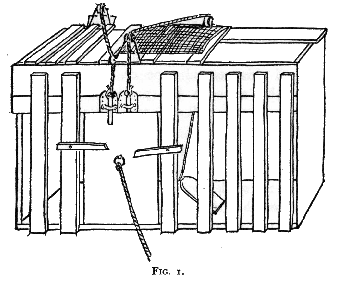
\includegraphics[width=0.7\linewidth]{puzzlebox.png}
  \caption{
    A puzzle box used by Thorndike in his experiments.
    The hungry cat is locked inside the box which it can open
    by solving some kind of puzzle
    in order to reach the fish outside.
    Results showed that the cat went from solving the puzzle by sheer happenstance
    to methodically opening it as if by habit.
  }
  \label{fig:puzzlebox}
\end{figure}

The psychological field of animal behavior and learning
has a longer history than the computational counterpart does,
with popular examples such as Pavlov's research.
The Russian Nobel laureate studied how animals
responded to different stimuli:

\begin{displayquote}
It is pretty evident that under natural conditions the normal animal must
respond not only to stimuli which themselves bring immediate benefit or harm,
but also to other physical or chemical agencies—waves of sound,
light, and the like—which in themselves only signal the approach of these stimuli;
though it is not the sight and sound of the beast of prey 
which is in itself harmful to the smaller animal, but its teeth and claws.
\attrib{\cite{pavlov1927conditional}, p. 14}
\end{displayquote}

In this same text the term "reinforcement"
was used for the first time in the context of animal learning.

Pavlov is most known for his experiment with dogs.
He noticed dogs would produce saliva in response
to receiving food.
He then associated a secondary stimulus to the act
of feeding the animals
by ringing a bell beforehand.
The dogs learned to associate the bell
with food and produced saliva
upon hearing the bell,
even before or without receiving anything.

\paragraph{}
Using trial-and-error to achieve artificial intelligence 
was among the earliest ideas in the field.
Alan Turing describes positive and negative stimuli
to influence an algorithm:

\begin{displayquote}
  When a configuration is reached for which the action is undetermined, a
random choice for the missing data is made and the appropriate entry is
made in the description, tentatively, and is applied. When a pain stimulus
occurs all tentative entries are cancelled, and when a pleasure stimulus
occurs they are all made permanent.

\attrib{\cite{turing1948intelligent}}
\end{displayquote}

Reinforcement Learning as I treat it here
solely means the computational approach
to learning from interaction,
except where mentioned explicitly.
We will not theorize on animal behavior
or try to model it in order to create computational models.
Sometimes, however,
inspiration is drawn from animal behavior
but it usually is no more than that;
analogies only go as far as they serve us.
The perspective used here is that of the engineer,
not the neuroscientist.

\paragraph{}
Central to reinforcement learning is that a learner
interacts with its environment in order to learn
and ultimately aims to achieve some goal.
Applied to human behavior in the course of a lifetime,
we could say humans -in general- try to optimize happiness.
Applied to something less daunting than the human condition,
a sculptor may try to optimize beauty
or expressivity of a sculpture,
learning along the way how to do so in the best possible way.
It is this goal-based interaction that forms the core
to reinforcement learning.

\paragraph{}
Reinforcement learning can be characterized
by three distinguishing features,
setting it apart from other fields of learning

\begin{description}
  \item[Closed loop]
    In order to learn, a learning agent must interact
    with the environment to collect the necessary information.
    However, each action changes the environment in a certain way
    and in turn influences the agent's future inputs.
    This forms a \textit{closed loop}.

  \item[Discovery]
    An agent is provided with no instructions on what actions to take
    and how this will impact the environment.
    It is to discover this itself.

  \item[Time factor]
    Consequences of an action can be delayed by an unknown amount of time.
    Even the reward signal can be received many time steps later.
    The agent is to figure out for itself
    how its actions relate temporally to consequences.
    
    A good example of this is the game of chess with only a reward signal
    at the end of a match, either positive or negative.
    Some moves during the game are probably more important
    than others and some more complicated,
    like traps that take multiple moves to set up.
    Yet all moves together are rewarded with only a single signal
    at the end of the match.
    It is for the agent to unravel and attribute
    its actions according to importance.
\end{description}

\subsection{Reinforcement Learning and Machine Learning}
As I tried to convey above,
a crucial aspect to reinforcement learning
is trial-and-error, learning from interactions
with an environment that is not necessarily known.
This makes reinforcement learning different from
\textit{supervised learning}
which is most associated with machine learning.
In a supervised setting,
a labeled example set is provided
for the learner to learn from.
Learning in this context means generalizing from the training set
so queries about data not in this set
can still be answered accurately.

Reinforcement learning is different
in that it takes on more of the problem;
a learning algorithm is not presented with data
but instead must gather it by interacting with the environment.
In doing so it must also make a tradeoff between exploration and exploitation,
a characterizing element to reinforcement learning.
A learning agent can either \textit{exploit}
what it knows to be the best action in order to achieve its goal,
thereby possibly ignoring alternative routes of action
that would have resulted in better results,
or choose to \textit{explore}
what impact its actions have on the environment.
Neither strategy can be followed exclusively
if one wants to learn anything worthwhile,
a good combination of both is always needed.

\paragraph{}
On the "opposite" side of supervised learning
is we call unsupervised learning,
which is about finding hidden patterns in unlabeled data.
The supervision gap between the two obviously pertains
to whether the data has been created in a supervised manner.
An illusion is created that there are two sides to machine learning,
though reinforcement learning does not seem to fit either.
Reinforcement learning is effectively a third machine learning paradigm.

\subsection{Applications (TODO)}
Reinforcement learning has been applied in a multitude of domains,
not only the ones immediately called to mind when thinking
of autonomous agents like physical robots of all kinds,
though those have definitely gained a lot of attention.

%TODO pff geen zin nu
\paragraph{}
Survey by \cite{Kober2013}

\paragraph{}
Talk about self-driving cars

With the surge of new techniques and faster machines
reinforcement learning has also gotten popular with the public.
%TODO self-driving cars


\section{Reinforcement Learning Framework}
\subsection{Agent and Environment}
There are only few components to the reinforcement learning problem.
The learner and actor is dubbed the agent and everything outside it the environment.
The agent perceives its environment and acts on it,
receiving a reward in return.
The latter is a numerical value
which the agent tries to gain as much as possible of
during its time interacting with the environment.
This interaction goes on continually:
observation followed by action followed by reward.
The goal of the agent is to maximize its accumulated reward
over the entire span of a task,
i.e. an instance of a problem.
In order for it to do so
it must learn to not only look to immediate rewards
but must also look to what the future has to offer.

\begin{figure}[ht]
	\center
	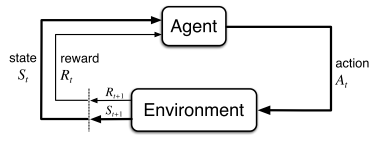
\includegraphics[width=.8 \linewidth]{agent-environment.png}
	\caption{The agent interacts with the environment and 
  consequentially perceives a reward and the next state of the environment.
  \parencite{Sutton1998a}
  }
	\label{agent-env}
\end{figure}

\paragraph{}
Formally, we divide the problem into discrete time steps $t$.
A time step occurs every time the agent perceives a state $S_t$
from the set of possible states $\mathcal{S}$.
Based on this state the agent selects an action $A_t$
from its repertoire of actions $\mathcal{A}(S_t)$
available to it at in state $S_t$.
As a result, the next step it will receive
a numerical reward $R_{t+1} \in \mathcal{R}$
along with the next state $S_{t+1}$,
and so on and so on.

\paragraph{}
As you can see, the problem setting is entirely abstract
and can be filled in in various ways.
In fact, the same practical problem may be defined in different ways
depending on the goal.
A state could just as well represent a robot's raw sensor readings
as well as higher-level representations
such as whether it is looking at a green or red light.
We say that state is provided by the environment
even though one could argue a robot's sensors
are part of the agent.
Instead, we look at the agent as the observer and decision-maker
taking in everything from a distance,
even its physical body external to it
as part of the environment.
Similarly to states,
actions can range from raw low-level values
like motor voltages
to higher-level concepts like which room to go to
or whether to turn left or right.
Basically, actions are decisions taken by the distant observer,
for the designer to decide which shape they take.

\paragraph{Cart Pole Balancing Example}
A popular experiment in reinforcement learning
that has its roots close to half a century ago
is the cart pole balancing experiment
\parencite{Michie1968}.

In this experiment,
a pole is affixed to a joint to the cart.
Because of the joint,
the pole can move in a two-dimensional plane
as shown in Figure \ref{fig:cartpole}.
The cart can move in two directions
parallel to the joint's movement.

Let us say the pole starts in a perfectly orthogonal
position to the cart.
However, because of the joint and
inherent material imperfections, however microscopic,
the pole will start to drop toward one side or the other.
It is now the cart's goal
to keep the pole balanced perfectly upward
by moving however it can.

\begin{figure}[ht]
  \centering
  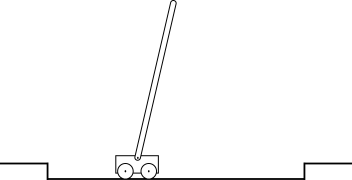
\includegraphics[width=0.7\linewidth]{cartpole.png}
  \caption{Cart Pole Experiment
  %TODO attribute to http://library.rl-community.org/wiki/CartPole_(Java)
  }
  \label{fig:cartpole}
\end{figure}

\paragraph{}
Applied to our framework,
we could at first glance say the cart is the obvious agent
and everything else its environment.
It would however make more sense
to name the textit{decision maker} that controls the cart the agent
and anything physical the environment or observable state.

As it is commonly defined,
a state exists of the angle of the pole with the cart
along with the angular velocity of the pole.
This would mandate three possible actions:
move left, move right, or stand still.

However, say the cart works in a more complicated manner
and actually has to accelerate instead of just
move at a fixed speed in one direction.
In that case,
the aforementioned state is insufficient
to correctly balance the pole;
car speed is now a crucial component
and should be added to the state if possible
to give a more complete description
and allow the agent to learn even better policies.
If not added, the agent will still learn
to the best of its abilities though.


\subsection{Goal and Rewards}
During a task,
an agent receives rewards upon acting with the environment.
Rewards can be positive or negative,
be real-valued or restricted to natural numbers,
the agent just has one goal with them.
There are different ways to define a goal.

\begin{description}
  \item[finite horizon] 
    The most naive way to collect rewards is through the
    \textit{finite-horizon} model,
    in which the agent aims to optimize its expected
    rewards for the next fixed amount of steps.
    This is rarely appropriate and still leaves us
    with the challenge of finding an appropriate value
    for the constant horizon window.
  \item[infinite horizon]
    The alternative then is to not have a fixed window
    but try to maximize reward over the rest of the agent's lifespan,
    albeit discounted so later rewards have less impact than current ones.
  \item[average reward]
    The average reward model makes the agent optimize
    its average reward over the rest of its lifetime.
    It relates closely to the infinite-horizon model, without the discount.
\end{description}

\begin{figure}[t]
  \centering
  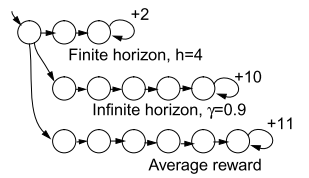
\includegraphics[width=0.5\linewidth]{optimality.png}
  \caption{Different goal models
  \parencite{Kaelbling1996} 
  }
  \label{fig:optimality}
\end{figure}

We will only ever use the \textit{infinite-horizon} model.

\section{Markov Decision Processes}
The Markov property is an interesting property for a problem to have
because it states that all relevant information at some point
is present in a state.
This means that the whole history leading up to a certain point,
insofar that it is relevant,
is encoded in the state at that time. 
Such a state is said to be Markov.

Formally, consider the probability of ending up in a state $s_{t+1}$
with reward $r_{t+1}$
after performing some action $a_t$
in a state $s_t$.
This probability is denoted

$$Pr(s_{t+1}=s', r_{t+1}=r | s_t, a_t)$$

We would say a state signal is Markov if this probability is the same as

$$Pr(s_{t+1}=s', r_{t+1}=r | s_t, a_t, s_{t-1}, a_{t-1},..., s_0, a_0)$$

which is the same scenario except given the entire state and action history. If these two are indeed equal, then the history is effectively encoded in the current state $s_t$.

\paragraph{}
START on mdp's here

\section{Value Functions}

\section{Temporal Difference Learning}

\section{Q-Learning}
Often we will discount future rewards
by a certain factor $\gamma$ per time step,
resulting in a total future discounted return
for the agent of
$R_t = \sum{T}{t'=t} \gamma^{t'-t}r_{t'}$,
with T the last time step.
This return is dependent on some policy $\pi$.
We now define $Q*(s,a)$ as the maximum expected return
when in a state s and taking action a.
This assumes we already know the optimal policy
in every subsequent state.
More formally,
$Q*(s,a) = max_{\pi}E[R_t|s_t=s, a_t=a, \pi]$

\paragraph{}
Since we assume we already know the optimal action in every state,
$$Q*(s,a) = E_{s'~\mathcal{E}}[r+\gamma max_{a'}Q*(s',a')|s,a]$$

Q-learning uses this equation directly
by plugging it into an iterative update.
Every step, the known Q-value for the visited state-action pair
is updated using a simple update rule:

$$<<TODO Q-learning update rule>>$$

with $\alpha$ a discount factor to stabilize the update.
This learned action	-value function directly approaches
the optimal action-value function $Q*$,
meaning that it always learns the optimal policy
of taking action $a' = argmax_{a}Q(s,a)$
in any state s.
The policy that is used to learn these Q-values
is only used for exploration purposes such that
sufficient state-action pairs are visited
and updated.
However, the policy itself is not optimized.
We call this off-policy learning,
as opposed to on-policy learning such as Sarsa-TD
where Q-values are updated with respect to
the currently used policy.
An advantage of Q-learning
is that it is guaranteed to converge
with probability 1
once certain conditions are fulfilled,
such as sufficiently small step size $\alpha$.

\paragraph{}
A problem with this learning approach is that
it enumerates all state-action pairs,
without generalization beyond visited pairs
and the added disadvantage of having to visit
each state-action pair multiple times
in order to have the Q-values converge.
Note that this makes the exploration strategy especially important,
as an agent that starts with a default Q-value assumption of 0
for each state-action pair can easily overfit
to non-zero Q-values if it is too greedy.
Moreover, and most importantly,
this approach does not scale well beyond only the smallest and most trivial
of state-action spaces.
This because the agent won't be able to enumerate all state-action pairs
sufficiently in such scenarios.
In the next section I will discuss how to alleviate this problem.

\section{Function Approximation}
To combat the problems brought along by a large state-action space,
we can use function approximators instead of storing Q-values
for each state-action pair,
which would quickly become infeasible.
To this end,
we could use any approximation method commonly used in machine learning
to approximate our state-action values.
However, reinforcement learning makes some methods
less suitable than others.
Samples gathered iteratively using reinforcement learning
usually have high correlation since an agent
takes a certain path through
the state-action space,
where neighboring states are usually somewhat similar.
The target to be learned is also not stationary,
since the real target value is often now known
but bootstrapped with some estimation.
For example,
in Q-learning the optimal action-value function $Q*$
is approximated using $r+\gamma max_{a'}Q(s',a')$
since we do not know the optimal $Q*$ in advanced.
This substituted target is still changing
because it has not been learned fully yet
and is both the value to be learned
as the target used for learning.
In subsequent sections I will discuss
how we can minimize the impact of these problems.
Still, it is important to be aware of them
when designing a function approximator.

\paragraph{}
One way of looking at the error of a Q-value approximator
with parameters $\theta$ is to look at the Mean Squared Error
between between the maximum expected return and
the predicted state-action value for all state-action pairs:
% formula kinda from sutton
% https://webdocs.cs.ualberta.ca/~sutton/book/ebook/node86.html
$$MSE(\theta) = \sum_{s \in S}[Q*(s,a)-Q(s,a,\theta)]^2$$
This error can then to be minimized over all samples
by a method such as gradient descent.

That is the traditional machine learning approach.
Note that reaching a global optimum for the parameters
is often only possible for linear functions
and not so anymore for more complex nonlinear functions.
In the harder case, we could instead look for local optima,
i.e. a case when $MSE(\theta') < MSE(\theta)$
for all $\theta$ near $\theta'$.

One should also be careful with simply minimizing the MSE
of the state-action function approximator
as our ultimate goal is to have the best policy $\pi$,
% TODO so.. do they collide? Sutton was vague at first	
two goals that do not necessarily collide.


\section{Eligibility Traces}
Valt te overwegen.

\section{Actor-Critic}

\chapter{Deep Reinforcement Learning}
Deep Learning describes a family of learning techniques
that at their core are about learning representations of data
in a hierarchical fashion.
It replaces the need for handcrafted feature
and indeed works in an entirely unsupervised or at least
semi-supervised fashion.
In this way,
it is often deployed as end-to-end learning
because it can learn its own higher-level abstractions
from raw data.

The core algorithm in deep learning is backpropagation
(described in detail in \ref{sec:backprop})
which describes how a learning model should update its parameters
in response to a discrepancy between learned output
and example output.

\paragraph{}
While the notion of stacking layers of units
to create multi-tiered artificial neural networks
has been around for a few decades already,
% TODO ref first Ann?
the recent surge in computing power
has enabled these conceptual models
to be actually built large enough
to explore their full potential.

Next to fully connected neural networks,
there are a few other types of networks of interest
that I will explore.
One such is the Convolutional Neural Network
which I will describe in more detail in
section \ref{sec:cnn}.
This type especially has benefitted from
advances in technology because of their highly
parallel nature which effectively allows them to be run
on consumer graphic hardware which is ever-improving
and becoming more accessible.

\paragraph{}
The areas that have benefited most from
this branch of machine learning
include without doubt
image recognition and speech recognition,
both problems with extremely noisy real-world data
that were typically tackled
by hand-crafting higher level features
and learning from those,
yet it is far from limited to these.
Deep learning has been extensively and successfully
applied to reinforcement learning as well,
the main topic of interest in this thesis.

\paragraph{}
The rest of this chapter will start by introducing
core deep learning conceps,
then proceed to applying deep learning
to the reinforcement learning case.
Sections \ref{sec:cnn} and \ref{sec:rnn}
concern themselves with general deep learning techniques,
i.e. not specific to the reinforcement learning.

% TODO add refs to later sections


\section{Convolutional Neural Networks}
\label{sec:cnn}
The core to deep learning is that representations
of data can be learned in an unsupervised manner.
Convolutional networks are able to learn features
from raw input without any human intervention.
Stacking convolutional layers even allows
hierarchical features to be learned.
This way the initial layer could function
as an edge detector
whereas deeper layers
would learn higher-level abstractions
such as for example facial features
in the case of image recognition.

Another core property of convolutional layers is that,
unlike a regular fully connected neural network,
it can recognize the same features
regardless of the location of the feature in the input.
A regular fully connected network would need to have
its weights in each of the possible locations trained to recognize the same feature
which is wasteful in both space and computational requirements.

\paragraph{}
Convolutional networks are strongly inspired
by the animal visual cortex which contains two basic cell types.
Simple cells activate respond most strongly to edge patterns;
they function as edge-detectors and have a small receptive field.
Complex cells on the other hands have a larger receptive field
and are also spatially invariant to pattern location.

An early predecessor of the convolutional network
that tried to capture these concepts
is the neocognitron
\parencite{Fukushima1980}
which differs mostly in that convolutional networks
share weights across several positions in the input,
as I will explain further down.
The architecture I will explain in the following section
is based on the famous LeNet-5,
designed by
\citeauthor{LeCun1998}
(\citeyear{LeCun1998})
to successfully recognize hand-written letters.

\section{Building Blocks}
\label{sec:building_blocks}

\subsection{Convolutional Layer}
The core building block for a convolutional network
is the convolutional layer.
For the remainder of this text it is easiest
to think of input as images, possibly
with a depth dimension (such as color).

\begin{figure}[htpb]
  \centering
  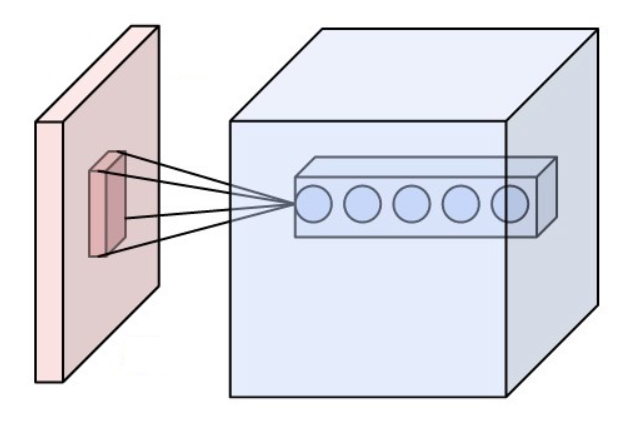
\includegraphics[width=0.7\linewidth]{conv_layer.png}
  \caption{Convolutional layer (blue) connected to an input layer.
    Highlighted are multiple filters connecting to a single input tile.
  }
  \label{fig:conv_layer}
\end{figure}

\paragraph{}
Let us start with the notion of a single, trainable neuron
in the convolutional layer.
It connects to only a small part of
the underlying input layer
as demonstrated in
Figure \ref{fig:conv_layer},
albeit through the whole depth.
This is the receptive field
as I described earlier.
Strongly connecting to only a small part of the input
is what allows convolutional networks
to exploit strong local correlations
that are inherently present
in natural images
but also in many other forms of
naturally occurring data.

\paragraph{}
This single neuron is part of a filter
that spans the whole input image,
it has neighbors that just like it
fully connect to neighboring patches of input.
One such a filter is now a flat 2D activation map
for a single feature.
This replication for a single filter
is what makes convolutional networks
insensitive to the location of a feature.

Of course we would like to have multiple features,
so we stack multiple of these filters on top of one another.
This stacking behavior of filters is described in
Figure \ref{fig:conv_layer},
where a single input patch is shown to correspond
to several filters.

\subsection{Parameter Sharing}
\label{sub:parameter_sharing}
As stated before, one feature corresponds to neurons across
the whole input by each corresponding to some patch of it.
This relies on the assumption that the feature could arise
anywhere in the input and would be useful to discover anywhere.
In order to actually compute the same feature,
we constrain the weights and bias of the neurons for a single feature
to be shared.

\subsection{Details}
\label{sub:details}
To actually generate the feature map
we \textit{convolve} the input with a linear filter,
add a bias and afterwards apply a non-linear function
such as a rectifier
(described in Section \ref{sec:relu}).
It is only because the weights are shared across a single feature
that this convolution is possible,
hence the name of the layer.

\paragraph{}
A single feature map $k$ in terms of its input $x$ could be computed as:

\begin{equation}
  h_k = tanh((W_k \cdot x) + b_k)
\end{equation}

It is also this operation that allows convolutional networks
to run so efficiently on parallel hardware,
making it the ideal candidate
for general purpose GPU computing.

\subsection{Tuning}
A single convolutional layer
has some hyperparameters that are both important
and hard to tweak.
Since learning a convolutional network
is still a rather slow endeavour,
it is best to start out with good estimates from the deep learning community.

\paragraph{}
The common way to build a convolutional network
from convolutional layers is to have
the layers closer to the input compute
few features,
computed over large receptive fields or tiles.
As the network grows deeper,
inputs to layers represent higher level features
and can thus be combined with less at a time;
intuitively, a few high-level features
can contain the same information of more
lower-level features.
Conversely, while there are only few
worthwhile raw features such as different types of edges,
there are probably more distinct higher-level features
that can be used to generate the final output.
Deeper layers should thus grow deeper yet slimmer spatially.

This setup typically results in a funnel-like structure
such as shown in Figure \ref{fig:conv_layer_funnel}.
The deepening occurs because of the increase in features
whereas the slimming usually occurs because multiple
outputs from an input layer correspond to only a single
neuron, spatially, in the next layer.
However, there are ways to train a neuron on a patch of input
yet still retain output size (again, spatially).
These I will describe below.

\begin{figure}[htpb]
  % TODO attribute to Hausknecht2015
  % TODO no seriously create new
  \centering
  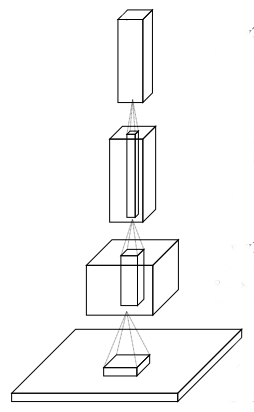
\includegraphics[width=0.3\linewidth]{conv_layer_funnel.png}
  \caption{Convolutional layers are often stacked
    in a funnel-like manner,
    growing smaller spatially
    yet larger in the depth or feature dimension.
  }
  \label{fig:conv_layer_funnel}
\end{figure}

\paragraph{}
As noted, both the amount of features
as well as the size of the receptive field in a layer
play a huge role in the representational capacity of the layer.
Still, there are other ways to affect this.
\begin{description}
  \item[Stride]
    The stride for a convolutional layer determines the spacing
    between receptive fields, or tiles.
    A stride of 1 would have very strongly overlapping tiles
    and as a result larger spatial dimensions
    than a lower stride would have.
    A stride equal to the tile size
    would result in non-overlapping but touching tiles.
    An even larger one would, of course,
    result in unused input elements and is therefore
    rather unpopular in practice.
  \item[Padding]
    If not all input elements can be used
    because of the filter size or the combination
    of filter size and stride,
    one can choose to pad the input with zeroes
    to achieve a valid convolution.
\end{description}

\subsection{Pooling Layer}
An important yet simpler concept to
convolutional networks is pooling,
a non-linear downsampling of the input.
The most popular form is max pooling,
demonstrated in Figure \ref{fig:maxpool}.

\begin{figure}[htpb]
  \centering
  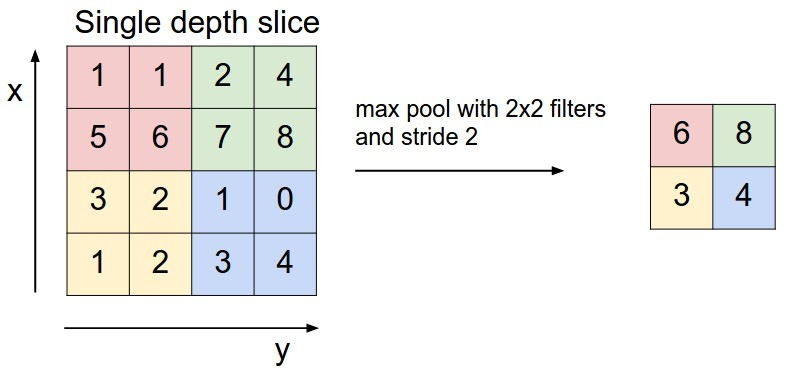
\includegraphics[width=0.7\linewidth]{maxpool.jpg}
  \caption{Max pooling with a filter size of $2 \times 2$
    and stride $2$.
  }
  \label{fig:maxpool}
\end{figure}

\paragraph{}
Pooling reduces the spatial size
while retaining the depth
as the depth describes the amount of features.
The idea behind the concept
is that spatial location of a feature is less important
than the activation of the feature
(note again the importance of translation invariance),
along with the notion that features are most important
in relation to other features.
Pooling therefore preserves relative location of each feature.

\paragraph{}
Even though most convolutional networks
tended to have pooling layers,
if not occasionally in between convolutional layers
then often right after them,
in recent years in the literature
there has been a tendency to avoid pooling layers altogether.
\citeauthor{Springenberg2015}
(\citeyear{Springenberg2015})
suggest that pooling does not always improve performance
if the network already has enough capacity for the data at hand
and indeed advocate the use of convolutional layers
with larger strides
and even more convolutional layer
to make up for the loss in power.

\section{Recurrent Neural Networks}
\label{sec:rnn}
Some tasks are sequential in nature,
meaning one sample depends on a previous one,
rather than data being independently
drawn from some unknown underlying distribution.
Typical problems include speech and language.

Recurrent neural networks are especially suited
for these domains.
They process input sequences one step at a time,
maintaining learned hidden state which will then
affect future output.
% TODO mention recurring connection

\paragraph{}
It is no wonder this class of artificial neural networks
draws the eye of the reinforcement learner designer.
A problem with a pure Markov state space
has no need of a network useful for learning dependencies between different states,
since by definition every state on its own is sufficient enough of a representation
and includes all necesary past states in its description.
However, many reinforcement learning problems are not strictly Markovian
and are only reduced to Markov decision processes for convenience.
Since these problems do not adhere strictly to Markovness,
they could still benefit from RNN's.

Recall also from section \ref{sub:pomdp}
the class of Partially Observable Markov Decision Procceses (POMDP).
These are processes that simply lack all required information in
at least some state descriptions.
As a result this is the class of problems that benefit most
from recurrent neural networks
and as a result are of special interest in this thesis.

\subsection{Building Blocks and Training}
\label{sub:building_blocks_and_training}
As Recurrent Neural Networks form a class of networks,
I will go over the general approach taken instead of a specific version.

Whereas regular feed-forward networks contain only forward connections,
RNN's usually contain cycles allowing them to capture time dependencies.
The cycle allows on state to depend on a previous one,
making it the ideal setup for sequences.

\begin{figure}[htpb]
  \centering
  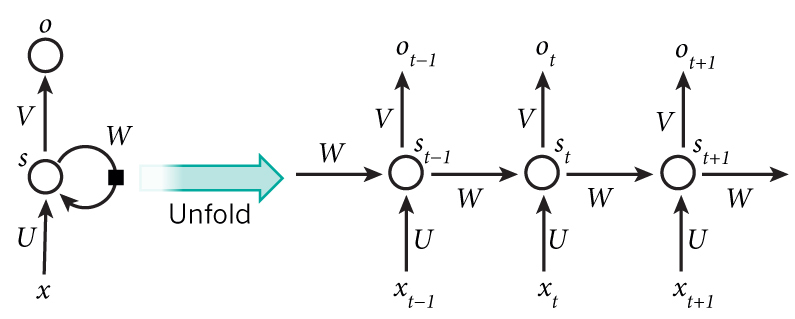
\includegraphics[width=0.8\linewidth]{rnn.jpg}
  \caption{Recurrent Neural Network unfolded through time
  \parencite{Y.2015dl}.
  }
  \label{fig:rnn}
\end{figure}

At first, it might look daunting to train a network with recurrent connections
and as a result a recursive component in the error.
However, recurrent neural networks can simply be trained with gradient descent.
Figure \ref{fig:rnn} shows how a recurrent connection can be viewed
throughout three different time steps.
Seen in this rolled out fashion,
it simply becomes a very deep network with shared weights
and allows us to apply the well-known backpropagation algorithm.

\subsection{Long Short-Term Memory Networks}
\label{sub:lstm}
Regular recurrent neural networks can suffer from two problems during training:
\textit{vanishing gradient} and {exploding gradient}.
Highlighted first by
\citeauthor{Bengio1994} (\citeyear{Bengio1994}),
these two recurring problematic phenomena have long prevented
efficient traiffic of recurrent neural networks.

The \textit{exploding gradient} describes the norm of the gradient
increasing during training
because of explosive growth of the long-term components
which then far outweigh the short-term components.
The opposite phenomenon, \textit{vanishing gradient},
features more prominently in the literature.
It describes long term components that go exponentially fast to zero,
making it practically impossible to learn
long-term time dependencies of arbitrary length.

To deal with the exploding gradient,
\parencite{Pascanu2012}
suggest clipping the norm of the gradients
and
% TODO pls verify with Peter
\citeauthor{Graves2013} (\citeyear{Graves2013})
show that \textit{skip connections},
i.e. connections that `skip' a layer,
help mitigate the vanishing gradient problem
for deep networks.

\paragraph{}
An architecture especially good at storing and accessing information
is the \textit{Long Short-Term Memory},
introduced by \citeauthor{Hochreiter1997} (\citeyear{Hochreiter1997}).
% TODO eh you sure?
It remedies extreme gradients
by enforcing a constant error flow through special internal units.
It also contains gates that regulate
which inputs get remembered or even forgotten,
as well as gates that regulate when to output a remembered value.

\begin{figure}[htpb]
  \centering
  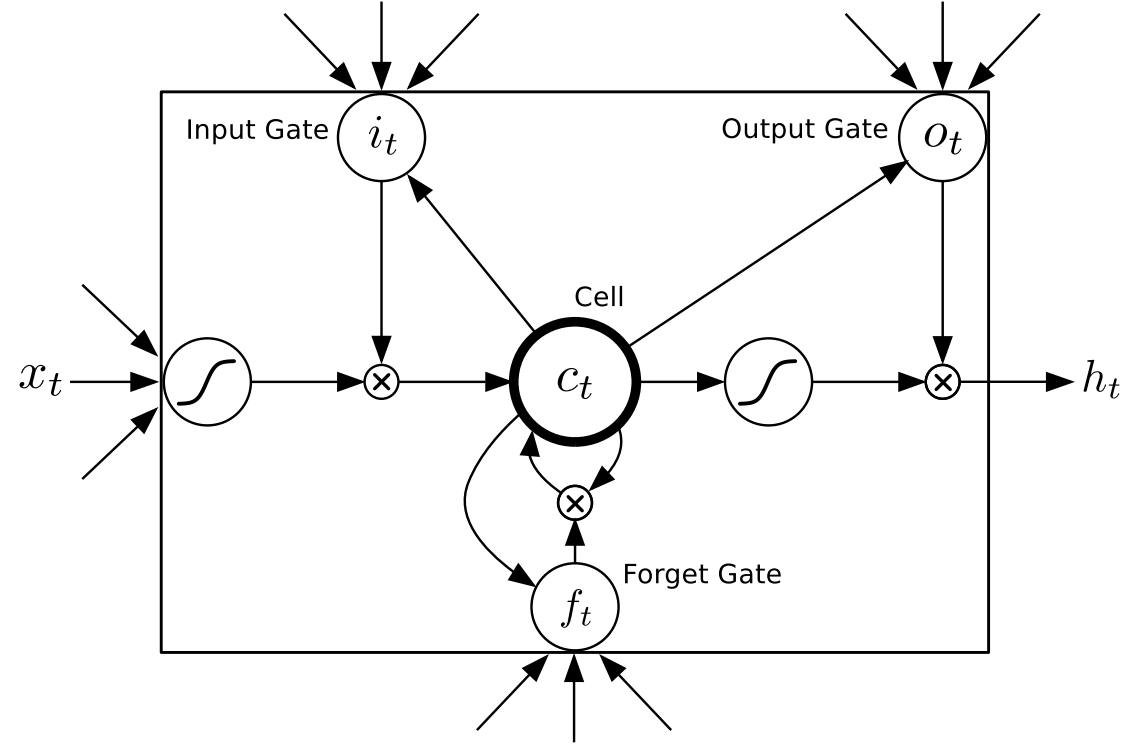
\includegraphics[width=0.8\linewidth]{lstm.png}
  \caption{Long Short-Term Memory cell
  \parencite{Graves2013}.
  }
  \label{fig:lstm}
\end{figure}

\paragraph{}
The basic unit is a Long Short-Term Memory cell
which is displayed schematically in Figure \ref{fig:lstm}.
A cell contains three gates:
an input gate, forget gate and output gate.
Each gate uses an activation function,
often the sigmoid function.
Central to it all is the cell unit, the internal state,
which gets regulated by the gates
in a fashion described by their names;
one gate controls whether the internal state should be overridden,
the other whether it should be used in the output
and yet another whether the internal state should be forgotten.
The combination of these elements make the LSTM cell into
into a veritable piece of memory.

\paragraph{}
The relations between the different components are described as follows,
where $\sigma$ is the sigmoid activation function:

\begin{align}
  &i_t = \sigma(W_{xi}x_t + W_{hi}h_{t-1}+W_{ci}c_{t-1} + b_i) \\
  &f_t = \sigma(W_{xf}x_t + W_{hf}h_{t-1}+W_{cf}c_{t-1} + b_f) \\
  &o_t = \sigma(W_{xo}x_t + W_{ho}h_{t-1}+W_{co}c_{t-1} + b_o) \\
  &c_t = f_tc_{t-1}+i_t tanh(W_{xc}x_t+W_{hc}h_{t-1}+b_c) \\
  &h_t = o_t tanh(c_t)
\end{align}

The $W_{ij}$ notation denotes the weights associated
with the connection from unit $i$ to unit $j$.
Likewise, $b_k$ denotes the bias for unit $k$.

While the equations might look daunting at first glance,
they can all be given intuitive meaning.
The three gates behave similarly;
they all depend on the current cell input ($x_t$),
the previous output ($h_{t-1}$)
and previous internal cell state ($c_{t-1}$).
All combine these inputs using a linear computation
and become non-linear through the activation function.

The internal cell state is a combination
of a `forget component' that determines
how the previous cell state is carried over
along with a combination of the current input and the previous output,
weighted by the current input gate
which regulates how the input should be used.

It must be noted that the original LSTM proposal
did not contain a forget gate
and simply added unchanged cell state
back into the current update.
This cell state was then referred to as the Constant Error Carousel (CEC),
named so because it enforced a constant error
in order to mitigate the vanishing and exploding gradient problems.



\section{Misc, still needs a decent place}
\subsection{RMSProp}
\label{sub:rmsprop}

\chapter{Experiments and Results}

\printbibliography
\end{document}
